\documentclass[border=8pt]{standalone}
\usepackage[T1]{fontenc}
\usepackage{amsmath,amssymb}
\usepackage{tikz}
\usetikzlibrary{calc,arrows.meta,positioning,decorations.pathreplacing,fit}

\definecolor{solvblue}{RGB}{200,220,245}
\definecolor{quasisolv}{RGB}{255,230,195}
\definecolor{combgreen}{RGB}{210,240,210}
\definecolor{emptycell}{RGB}{240,240,240}
\definecolor{axislabel}{RGB}{60,60,60}
\definecolor{darkblue}{RGB}{40,80,140}
\definecolor{darkorange}{RGB}{160,100,20}
\definecolor{darkgreen}{RGB}{40,120,60}
\definecolor{arrowred}{RGB}{180,50,50}

\begin{document}
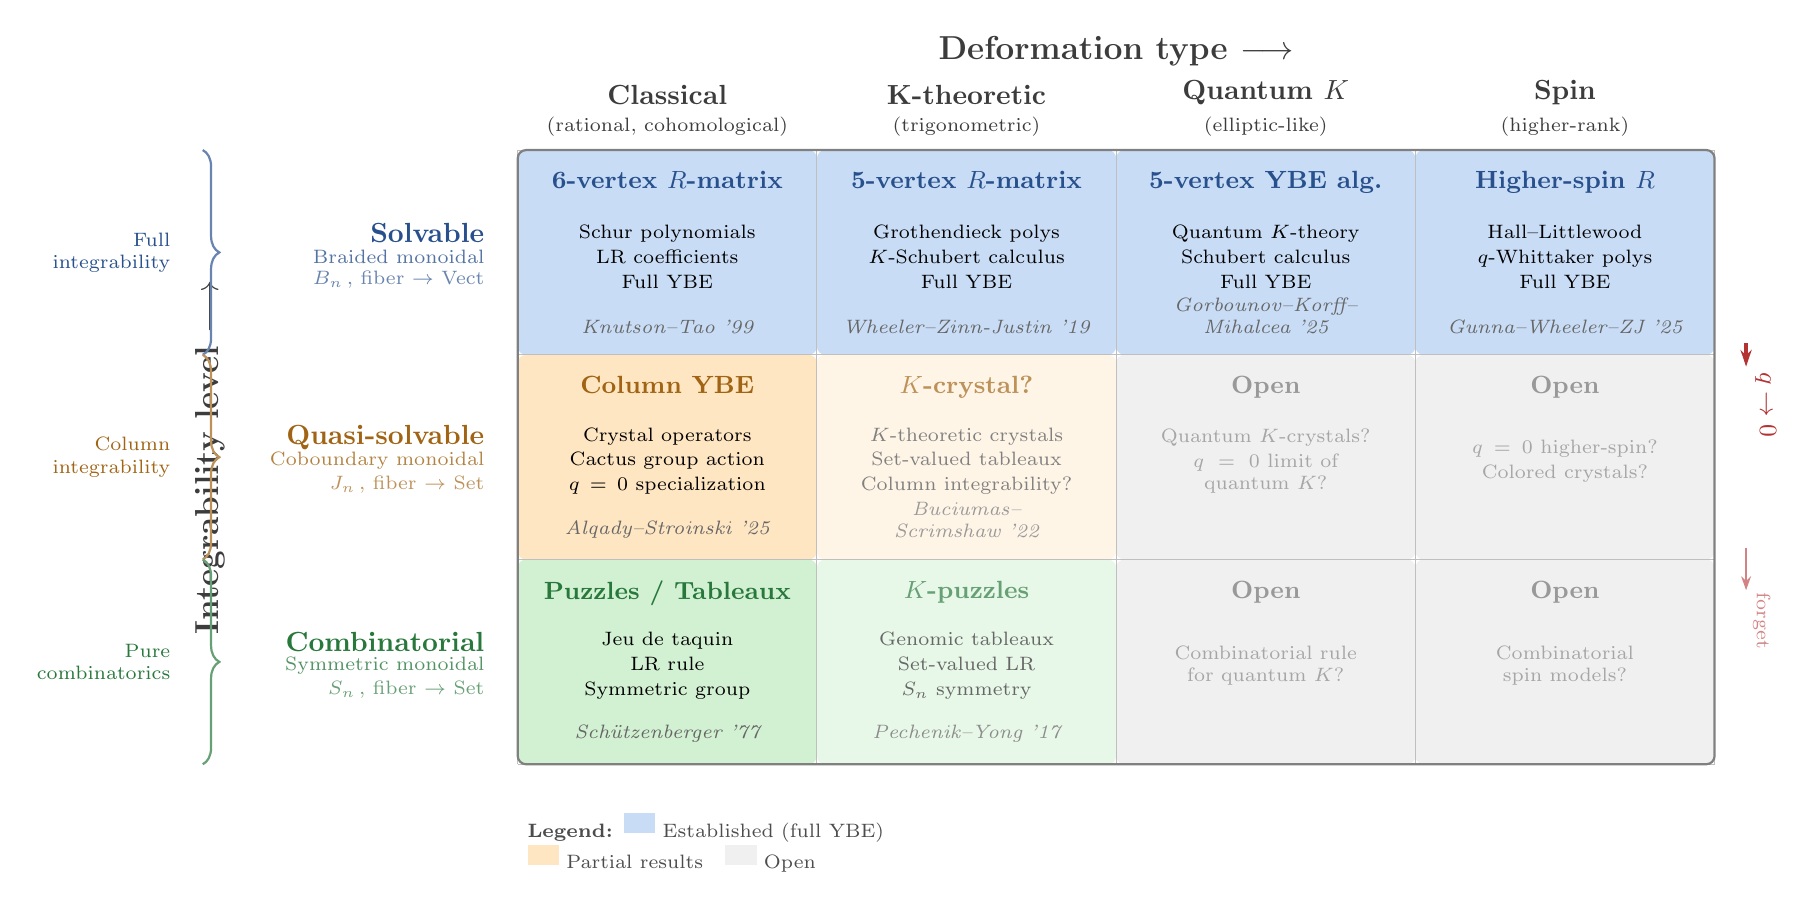
\begin{tikzpicture}[
    every node/.style={font=\small},
    celltitle/.style={font=\bfseries\small, anchor=north},
    cellref/.style={font=\scriptsize\itshape, text=black!60, anchor=south, text width=3.2cm, align=center},
    cellbody/.style={font=\scriptsize, anchor=center, text width=3.2cm, align=center},
    axistitle/.style={font=\bfseries\normalsize, text=axislabel},
]

% Dimensions
\def\cw{3.8}  % cell width
\def\ch{2.6}  % cell height
\def\cols{4}
\def\rows{3}

% =====================================================================
% Column headers
% =====================================================================
\foreach \j/\hdr/\sub in {
  0/{Classical}/{(rational, cohomological)},
  1/{K-theoretic}/{(trigonometric)},
  2/{Quantum $K$}/{(elliptic-like)},
  3/{Spin}/{(higher-rank)}%
}{
  \node[axistitle, anchor=south] at ({\j*\cw+\cw/2}, {\rows*\ch+0.45}) {\hdr};
  \node[font=\scriptsize, text=axislabel, anchor=south] at ({\j*\cw+\cw/2}, {\rows*\ch+0.05}) {\sub};
}

% Horizontal axis label
\node[font=\bfseries\large, text=axislabel] at ({2*\cw}, {\rows*\ch+1.25})
  {Deformation type $\longrightarrow$};

% =====================================================================
% Row labels (right side, to leave room for vertical axis label)
% =====================================================================
\foreach \i/\lbl/\cat/\grp/\fiber/\col in {
  2/{Solvable}/{Braided monoidal}/{$B_n$}/{$\mathrm{Vect}$}/darkblue,
  1/{Quasi-solvable}/{Coboundary monoidal}/{$J_n$}/{$\mathrm{Set}$}/darkorange,
  0/{Combinatorial}/{Symmetric monoidal}/{$S_n$}/{$\mathrm{Set}$}/darkgreen%
}{
  % Row name
  \node[axistitle, anchor=east, text=\col] at (-0.3, {\i*\ch+\ch/2+0.25}) {\lbl};
  % Categorical annotation
  \node[font=\scriptsize, anchor=east, text=\col!80] at (-0.3, {\i*\ch+\ch/2-0.05}) {\cat};
  % Group and fiber functor
  \node[font=\scriptsize, anchor=east, text=\col!70] at (-0.3, {\i*\ch+\ch/2-0.35}) {\grp\,,\ fiber $\to$ \fiber};
}

% Vertical axis label
\node[font=\bfseries\large, text=axislabel, rotate=90, anchor=south]
  at (-3.6, {\rows*\ch/2})
  {Integrability level $\longrightarrow$};

% =====================================================================
% Draw cells — row 2 = solvable (top), row 1 = quasi, row 0 = comb
% =====================================================================

% --- Solvable row (blue) ---
% (0,2) Classical / Solvable
\fill[solvblue, rounded corners=3pt] (0,{2*\ch}) rectangle ++(\cw,\ch);
\node[celltitle, text=darkblue] at (\cw/2, {3*\ch-0.15}) {6-vertex $R$-matrix};
\node[cellbody] at (\cw/2, {2*\ch+\ch/2-0.05}) {Schur polynomials\\[1pt] LR coefficients\\[1pt] Full YBE};
\node[cellref] at (\cw/2, {2*\ch+0.15}) {Knutson--Tao '99};

% (1,2) K-theoretic / Solvable
\fill[solvblue, rounded corners=3pt] (\cw,{2*\ch}) rectangle ++(\cw,\ch);
\node[celltitle, text=darkblue] at ({1.5*\cw}, {3*\ch-0.15}) {5-vertex $R$-matrix};
\node[cellbody] at ({1.5*\cw}, {2*\ch+\ch/2-0.05}) {Grothendieck polys\\[1pt] $K$-Schubert calculus\\[1pt] Full YBE};
\node[cellref] at ({1.5*\cw}, {2*\ch+0.15}) {Wheeler--Zinn-Justin '19};

% (2,2) Quantum K / Solvable
\fill[solvblue, rounded corners=3pt] ({2*\cw},{2*\ch}) rectangle ++(\cw,\ch);
\node[celltitle, text=darkblue] at ({2.5*\cw}, {3*\ch-0.15}) {5-vertex YBE alg.};
\node[cellbody] at ({2.5*\cw}, {2*\ch+\ch/2-0.05}) {Quantum $K$-theory\\[1pt] Schubert calculus\\[1pt] Full YBE};
\node[cellref] at ({2.5*\cw}, {2*\ch+0.15}) {Gorbounov--Korff--Mihalcea '25};

% (3,2) Spin / Solvable
\fill[solvblue, rounded corners=3pt] ({3*\cw},{2*\ch}) rectangle ++(\cw,\ch);
\node[celltitle, text=darkblue] at ({3.5*\cw}, {3*\ch-0.15}) {Higher-spin $R$};
\node[cellbody] at ({3.5*\cw}, {2*\ch+\ch/2-0.05}) {Hall--Littlewood\\[1pt] $q$-Whittaker polys\\[1pt] Full YBE};
\node[cellref] at ({3.5*\cw}, {2*\ch+0.15}) {Gunna--Wheeler--ZJ '25};

% --- Quasi-solvable row (orange) ---
% (0,1) Classical / Quasi-solvable
\fill[quasisolv, rounded corners=3pt] (0,\ch) rectangle ++(\cw,\ch);
\node[celltitle, text=darkorange] at (\cw/2, {2*\ch-0.15}) {Column YBE};
\node[cellbody] at (\cw/2, {\ch+\ch/2-0.05}) {Crystal operators\\[1pt] Cactus group action\\[1pt] $q=0$ specialization};
\node[cellref] at (\cw/2, {\ch+0.15}) {Alqady--Stroinski '25};

% (1,1) K-theoretic / Quasi-solvable
\fill[quasisolv!40, rounded corners=3pt] (\cw,\ch) rectangle ++(\cw,\ch);
\node[celltitle, text=darkorange!70] at ({1.5*\cw}, {2*\ch-0.15}) {$K$-crystal?};
\node[cellbody, text=black!50] at ({1.5*\cw}, {\ch+\ch/2-0.05}) {$K$-theoretic crystals\\[1pt] Set-valued tableaux\\[1pt] Column integrability?};
\node[cellref, text=black!40] at ({1.5*\cw}, {\ch+0.15}) {Buciumas--Scrimshaw '22};

% (2,1) Quantum K / Quasi-solvable — open
\fill[emptycell, rounded corners=3pt] ({2*\cw},\ch) rectangle ++(\cw,\ch);
\node[celltitle, text=black!40] at ({2.5*\cw}, {2*\ch-0.15}) {Open};
\node[cellbody, text=black!35] at ({2.5*\cw}, {\ch+\ch/2-0.05}) {Quantum $K$-crystals?\\[1pt] $q=0$ limit of\\quantum $K$?};

% (3,1) Spin / Quasi-solvable — open
\fill[emptycell, rounded corners=3pt] ({3*\cw},\ch) rectangle ++(\cw,\ch);
\node[celltitle, text=black!40] at ({3.5*\cw}, {2*\ch-0.15}) {Open};
\node[cellbody, text=black!35] at ({3.5*\cw}, {\ch+\ch/2-0.05}) {$q=0$ higher-spin?\\[1pt] Colored crystals?};

% --- Combinatorial row (green) ---
% (0,0) Classical / Combinatorial
\fill[combgreen, rounded corners=3pt] (0,0) rectangle ++(\cw,\ch);
\node[celltitle, text=darkgreen] at (\cw/2, {\ch-0.15}) {Puzzles / Tableaux};
\node[cellbody] at (\cw/2, {\ch/2-0.05}) {Jeu de taquin\\[1pt] LR rule\\[1pt] Symmetric group};
\node[cellref] at (\cw/2, 0.15) {Sch\"utzenberger '77};

% (1,0) K-theoretic / Combinatorial
\fill[combgreen!50, rounded corners=3pt] (\cw,0) rectangle ++(\cw,\ch);
\node[celltitle, text=darkgreen!70] at ({1.5*\cw}, {\ch-0.15}) {$K$-puzzles};
\node[cellbody, text=black!60] at ({1.5*\cw}, {\ch/2-0.05}) {Genomic tableaux\\[1pt] Set-valued LR\\[1pt] $S_n$ symmetry};
\node[cellref, text=black!45] at ({1.5*\cw}, 0.15) {Pechenik--Yong '17};

% (2,0) Quantum K / Combinatorial — open
\fill[emptycell, rounded corners=3pt] ({2*\cw},0) rectangle ++(\cw,\ch);
\node[celltitle, text=black!40] at ({2.5*\cw}, {\ch-0.15}) {Open};
\node[cellbody, text=black!35] at ({2.5*\cw}, {\ch/2-0.05}) {Combinatorial rule\\for quantum $K$?};

% (3,0) Spin / Combinatorial — open
\fill[emptycell, rounded corners=3pt] ({3*\cw},0) rectangle ++(\cw,\ch);
\node[celltitle, text=black!40] at ({3.5*\cw}, {\ch-0.15}) {Open};
\node[cellbody, text=black!35] at ({3.5*\cw}, {\ch/2-0.05}) {Combinatorial\\spin models?};

% =====================================================================
% Grid lines
% =====================================================================
\foreach \j in {0,...,4}{
  \draw[black!25] ({\j*\cw}, 0) -- ({\j*\cw}, {\rows*\ch});
}
\foreach \i in {0,...,3}{
  \draw[black!25] (0, {\i*\ch}) -- ({\cols*\cw}, {\i*\ch});
}
% Outer border
\draw[black!50, thick, rounded corners=3pt] (0,0) rectangle ({\cols*\cw}, {\rows*\ch});

% =====================================================================
% q -> 0 arrow between solvable and quasi-solvable rows
% =====================================================================
\draw[arrowred, -{Stealth[length=6pt,width=4pt]}, line width=1.5pt]
  ({\cols*\cw+0.4}, {2*\ch+0.15}) -- ({\cols*\cw+0.4}, {\ch+\ch-0.15});
\node[font=\bfseries\small, text=arrowred, anchor=west, rotate=-90]
  at ({\cols*\cw+0.65}, {2*\ch-0.1}) {$q \to 0$};

% Arrow between quasi-solvable and combinatorial
\draw[arrowred!60, -{Stealth[length=5pt,width=3.5pt]}, line width=1pt]
  ({\cols*\cw+0.4}, {\ch+0.15}) -- ({\cols*\cw+0.4}, {0.85*\ch});
\node[font=\small, text=arrowred!60, anchor=west, rotate=-90]
  at ({\cols*\cw+0.6}, {\ch-0.3}) {\scriptsize forget};

% =====================================================================
% Legend
% =====================================================================
\node[anchor=north west, font=\scriptsize, text=black!70, text width=5cm]
  at (0, -0.5) {%
  \textbf{Legend:}
  \tikz[baseline=-0.5ex]{\fill[solvblue] (0,0) rectangle (0.4,0.25);} Established (full YBE)\quad
  \tikz[baseline=-0.5ex]{\fill[quasisolv] (0,0) rectangle (0.4,0.25);} Partial results\quad
  \tikz[baseline=-0.5ex]{\fill[emptycell] (0,0) rectangle (0.4,0.25);} Open
  };

% =====================================================================
% Categorical flow annotation (left brace)
% =====================================================================
\draw[decorate, decoration={brace, amplitude=6pt, mirror}, darkblue!70, thick]
  (-4.0, {2*\ch}) -- (-4.0, {3*\ch})
  node[midway, left=8pt, font=\scriptsize, text=darkblue, align=right] {Full\\integrability};

\draw[decorate, decoration={brace, amplitude=6pt, mirror}, darkorange!70, thick]
  (-4.0, {\ch}) -- (-4.0, {2*\ch})
  node[midway, left=8pt, font=\scriptsize, text=darkorange, align=right] {Column\\integrability};

\draw[decorate, decoration={brace, amplitude=6pt, mirror}, darkgreen!70, thick]
  (-4.0, 0) -- (-4.0, {\ch})
  node[midway, left=8pt, font=\scriptsize, text=darkgreen, align=right] {Pure\\combinatorics};

\end{tikzpicture}
\end{document}
